In this chapter, the classical version of PMCLP using disks will be defined and a version of the method will be proposed with the intention of later being used to solve the axis-parallel ellipses version of PMCLP. Throughout the course of this work, the maximal covering by disks problem is going to be referred to as $MCD(\Pp,m)$ where $\Pp$ is a set of points and $m$ is the number of unit disks.

\section{One disk, $MCD(\Pp,1)$}


Two exact methods for the $MCD(\Pp, 1)$ have been found in the literature. A $\bigO(n^2)$ algorithm is proposed by \cite{chazelle:1986} which improved the previously $\bigO(n^2\log{n})$ one proposed by \cite{drezner}.
As it has been mentioned, $MCD(\Pp,1)$ is a 3SUM-HARD problem, which means that it is as hard as the 3SUM problem (the problem of finding $3$ real number that sum to $0$, given $n$ real numbers). Initially the lower bound of the 3SUM problem was conjectured to be $\Omega(n^2)$, matching the best algorithm for $MCD(\Pp,1)$, which meant that no better time-complexity could be achieved. Since then, however, better algorithms for 3SUM have been developed with a $\bigO(\frac{n^2}{poly(n)})$ run time complexity \cite{3SUM-kopelowitz:2014}.

The $m=1$ version is treated here before the general case because it will be shown that, using the algorithm here proposed for $MCD(\Pp, 1)$, an optimal solution can be obtained for the $MCD(\Pp, m)$ as well as for the axis-parallel ellipse version of the problem.

\subsection{Notation and definition of the problem}

Initially, the input of the problem defines a unit disk with its center point undefined, a solution for the problem will then choose a point to be the center of the unit disk, in other words a solution places the disk somewhere in the plane.
We refer to the unit disk with undefined center as $D$. If it is placed at a center $q \in \R^2$, we call it $D(q)$.

\begin{definicao}
    Let $\Pp=\{p_1,\dots,p_n\}$ be a set of $n$ points in $\R^2$, and $w(p)>0, p \in \Pp$ the weight of every point in $\Pp$, we denote $w(A)$, with $A \subset \Pp$, as the sum of weights of every point in $A$. Finally, let $D$ be a unit disk, we define the optimal solution of $MCD(\Pp,1)$ as
    
    \begin{equation}\label{eq:max_one_disk}
        \max_q w(\Pp \cap D(q))
    \end{equation}

\end{definicao}

Therefore, an optimal solution for an instance of $MCD(\Pp,1)$ will be a point in which a unit disk located at it, covers points whose weights, when summed, is maximal. 

In \cite{drezner}, the main idea used to develop the $\bigO(n^2\log{n})$ algorithm is that, even though there are infinitely many points where the disk could be placed, only a few of them, a finite amount of $\bigO(n^2)$, needs to be considered for the method to find an optimal one.
The algorithm, for every point, sorts the other points with respect to the angle they form with the first one. After that, the first point is placed on the border of the disk and, going through the sorted list, the algorithm inserts and removes points from the disk coverage. Also, when inserting and removing a point from the coverage, it only checks the disk centers that make the entering/leaving point to be on the border. Because the algorithm only checks the centers that make the disk have two points on its border, the number of centers it goes through is bounded by the number of pairs of points, which is $\binom{n}{2} = \bigO(n^2)$.

In \cite{chazelle:1986, cabello:2006}, on the other hand, the authors instead of working directly with $MCD(P,1)$, introduced an equivalent problem called maximum weight clique. Both methods for this problem consist on building a planar graph on which the vertices were the $\bigO(n^2)$ pairwise intersection of the circumferences and the edges were the arcs of the circumferences connecting the intersections. With the graph constructed, a traversal would be done to obtain the answer, thus the time complexity of $\bigO(n^2)$.
The algorithm that we later describe in this work also uses this equivalence. That is why it has been taken to be fundamental to introduce the maximum weight clique problem and discuss the equivalence.

\section{Maximum weight clique}

Let $\Pp=\{p_1,\dots,p_n\}$, with $p\in \R^2$ be a set of points, $\D=\{D_1,\dots,D_n\}$ a set of unit disks, such that $D_i$ is centered at $p_i$, $i=1,\dots,n$, with every disk having a weight $w_i > 0$, $i=1,\dots,n$. A clique, in this context, is a non-empty intersection area of a subset of disks. Note that this is different than the clique problem on a intersection graph (a graph where the vertices are the disks and an edge exists if there is an intersection between two disks). As shown in \autoref{fig:three_disks_no_intersection}, three disks could have non-empty pairwise intersection (which qualifies them as a clique), but the intersection of all the three together is empty. That is why the clique problem for unit disks is also referred to as the maximum geometric clique problem when the condition of common intersection exists and as the maximum graphical clique problem where there is only the pairwise intersection condition \cite{inplace:2014}. The graphical version of the problem was studied by \cite{graphical-clique} where a $\bigO(n^{4.5})$ algorithm was proposed. Also, in \cite{inplace:2014}, a $\bigO(n^2\log{n})$ time in-place algorithm, which needs $\bigO(1)$ extra space, for arbitrary radii disks was proposed.

\begin{figure}[H]
\centering

    \caption{Three disks that have non-empty pairwise intersection among them, but no common intersection}
    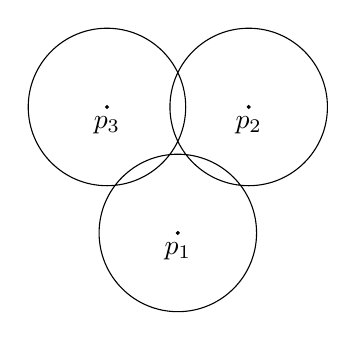
\begin{tikzpicture}[domain=0:11]
    %\draw [help lines] (-5,-3) grid (5,3);
    \draw (0,0) circle (1cm) (0.9,1.6) circle (1cm) (-0.9,1.6) circle (1cm);

    %a^2-b^2=c^2 -> c^2=25-9=16 -> c=4
    
    \draw[fill] (0.9,1.6) circle [radius=.5pt];
	\draw[fill] (0,0) circle [radius=.5pt];
    \draw[fill] (-0.9,1.6) circle [radius=.5pt];
    
    \node[below] at (0,0) {$p_1$};
    \node[below] at (0.9, 1.6) {$p_2$};
    \node[below] at (-0.9, 1.6) {$p_3$};
    
    %\draw [-] (-5,0) -- (5,0);
     %\draw [-] (0,-3) -- (0,3);
     %\draw [|-|] (0.001,-0.1) -- (4.999,-0.1);
    \end{tikzpicture}
    \label{fig:three_disks_no_intersection}
    \fautor
\end{figure}


A solution for the maximum weight clique is a set of points $Q$, such that the sum of weights of all disks that cover it is maximized. Even though, there could be a use for the whole set $Q$, as this problem is used as a tool to solve another problem, only finding a point from the maximum weight clique is enough. This will become clear when the equivalence is stated. With everything in hands, we can define the maximum weight clique problem as follows

\begin{definicao}\label{def:max_weight_clique}
    Let $\D$ be a set of unit disks and $\Pp$ be a set of points as defined before, an optimal solution for the maximum weight clique problem is given by 
    
    \begin{equation}
        \max_q \sum_{D_k \cap q \neq \emptyset} w_k
    \end{equation}

\end{definicao}

As it has been proposed, with the equivalence of the two problems, the optimal solution of the maximum weight clique problem is also the optimal solution of the $MCD(\Pp,1)$, which means that a disk centered at $q$, defined in \autoref{def:max_weight_clique}, will have a maximal weight covering of the set $\Pp$.

Given an instance of $MCD(\Pp,1)$, the equivalent maximum weight clique problem is obtained by defining the set $\D$ to be the disks centered at $\Pp$ and setting the weight of every disk to be the weight of its corresponding point in $\Pp$. A disk $D_i$ will represent the area where a disk can be placed in order to cover $p_i$, this means that a intersection between some disks is an area where a disk could be placed to cover the corresponding points.

In \autoref{fig:three_disks_no_intersection}, it can be seen that there is no point where a disk could be placed such that it would cover $p_1, p_2$ and $p_3$, nonetheless anywhere, in any of the pairwise intersections, a disk could be placed to cover the two corresponding points.

Formally, in the maximum weight clique problem, if a point $q$ lies inside $\bigcap_{k \in I} D_k$, with $I \subset \{1,\dots,n\}$, then a disk centered at $q$ will cover the points $p_k$, with $k\in I$ in the $MCD(P,1)$ problem. Conversely, the same applies for a disk placed at $q$ that covers points $p_k$, with $k \in I$ in the one disk maximal covering problem. It means that $q$ will lie inside the region $\bigcap_{k \in I} D_k$.

\subsection{An algorithm for the maximum weight clique problem}

The algorithm described here is based on the one in \cite{drezner}, also with some ideas from \cite{inplace:2014} and \cite{cabello:2006}. It has a run time complexity of $\bigO(n^2\log{n})$ and uses $\bigO(n)$ of extra space. It is worth noting, however, that a $\bigO((n+K)\log{n})$ run time, with $K$ being the number of intersections, can be obtained by using the algorithm in \cite{bentley:1979} to find all the intersections among the $n$ circumferences.

Without loss of generality, the weights will be ignored, and the method will be described for the maximum clique problem, assuming that every disk has unit weight. Also, it will be assumed that no pair of disks are placed at the same center.

Let $\D$ be a set of $n$ unit disks, a non-empty intersection area of a subset of disks is convex and bounded by the arcs of the disks that are intersecting \cite{inplace:2014}.
This observation makes checking for every disk $\Cc$, every intersection area that is bounded by its arc sufficient in order to find the optimal solution.

\begin{definicao}\label{def:inter_arc}
    Let $D_i$ and $D_j$ be two unit disks that intersect (at least at one point). Also let $(\theta_1, \theta_2) \in [0,2\pi]^2$ be the two angles that the circumferences induced by $D_i$ and $D_j$ intersect, with the condition that $(\theta_1,\theta_2)$ defines an arc (counter-clockwise order) of $D_i$ that is the border of $D_i \cap D_j$. If $D_i$ is tangent to $D_j$, then $\theta_1=\theta_2$. Then, We define $\Gamma_+(i,j) = \theta_1$ and $\Gamma_-(i,j) = \theta_2$, also we refer to them as opening and closing intersection angles respectively.
\end{definicao}

\begin{figure}[H]
\centering

    \caption{Three disks and their intersection points}
    \begin{tikzpicture}
%\draw [help lines] (-5,-3) grid (5,3);

\draw[name path = c1] (0,0) circle (1cm);
\draw[name path = c3] (0.6,-0.82) circle (1cm);
\draw[name path = c2] (-0.4,-0.82) circle (1cm);

\node[above] at (0, 1) {$D_1$};
\node[left] at (-1.4, -0.82) {$D_2$};
\node[right] at (1.6, -0.82) {$D_3$};

\path [name intersections={of=c1 and c3}] ;
\foreach \i in {1,...,2}
\fill [color=gray] (intersection-\i) circle (2pt) ;

\node[right] at (intersection-1) {\tiny $\Gamma_-(1,3)$};
\node[left, below] at (intersection-2) {\tiny $\Gamma_+(1,3)$};

\path [name intersections={of=c1 and c2}] ;
\foreach \i in {1,...,2}
\fill [color=gray] (intersection-\i) circle (2pt) ;

\node[left] at (intersection-1) {\tiny $\Gamma_+(1,2)$};
\node[below,right] at (intersection-2) {\tiny $\Gamma_-(1,2)$};

%\draw [-] (-5,0) -- (5,0);
%\draw [-] (0,-3) -- (0,3);
%\draw [|-|] (0.001,-0.1) -- (4.999,-0.1);
\end{tikzpicture}
    \fautor
    \label{fig:3disks_intersect}
\end{figure}

In \autoref{fig:3disks_intersect}, it is shown all the intersection points between $D_1$ with $D_2$ and $D_3$, also they are labeled according to \autoref{def:inter_arc}, note that $\Gamma_+(1,3) > \Gamma_-(1,3)$ (the angles should be in the $[0,2\pi]$ interval).

With \autoref{def:inter_arc} in hands, we can establish the basis of the algorithm to find the maximum clique that a disk $D_i$ participates: a traversal going through every point of intersection with $D_i$ in counter-clockwise order keeping a set of active disks, when an opening intersection angle is reached, the corresponding disk is added to the active set; when a closing one is reached, the corresponding disk is removed from the active set.
This simple traversal, however, would not handle the special case with $\Gamma_+(i,j) > \Gamma_-(i,j)$, see \autoref{fig:3disks_intersect}. If the traversal begins at the point with smallest angle, the algorithm would remove $D_3$ from the active disks without first adding it, if there was another disk starting before $\Gamma_-(1,3)$, the algorithm would not have both of them in the active set at the same time, and the optimal solution could end up not being found. This can be worked around repeating the traversal once without resetting the active disks set, that way in the beginning of the second traversal, the active set would contain the disks that have $\Gamma_+(i,j) > \Gamma_-(i,j)$.


\begin{algoritmo}
\caption{Algorithm for $MCD(\Pp, 1)$ with unit weights}\label{algoritmo:mcd_1}
\begin{algorithmic}[1]
\Procedure{$MCD_1$}{$\Pp$}\Comment{Returns the maximum number of disks that have a non-empty.}
\State $Q_{best} \gets \{\}$
\State $ans \gets$ center of $D_1$
\ForAll{$p_i \in \Pp$}
\State Let $D_i$ be the disk with center at $p_i$
\State Let $I_i$ be the set of disks that intersect with $D_i$
\State $A = \bigcup_{j \in I_i} \Gamma_+(i,j) \cup \Gamma_-(i,j)$

\State $Q \gets \{D_i\}$ \Comment{The set of active disks}
\For{$cnt=1..2$} \Comment{Do it twice}
\For{$a \in A$}\Comment{Assuming $A$ is sorted}
\State Let $D_a$ be the disk that intersects $D_i$ at angle $a$. 
\If{$a$ is a starting angle}
\State $Q \gets Q \cup \{D_a\}$
\Else
\State $Q \gets Q \setminus \{D_a\}$
\EndIf
\If{$|Q_{best}| < |Q|$}
\State $Q_{best} \gets Q$
\State $ans \gets $ point corresponding to the intersection angle $a$
\EndIf
\EndFor
\EndFor
\EndFor

\State \Return $ans$
\EndProcedure
\end{algorithmic}
\end{algoritmo}

\begin{lema}\label{lema:disk}
The \autoref{algoritmo:mcd_1} for the maximum clique has a $\bigO((n+K)\log{n})$ run time complexity where $K$ is the number of intersections of the $n$ disks.
\end{lema}

\begin{proof}
    Finding every intersection can be done in $\bigO((n+K)\log{n})$  by a plane sweep, the method is described in \cite{bentley:1979}. 
    Because the traversal is made in counter-clockwise order, the intersection points have to be sorted by their intersection angles, so an additional $\bigO(K\log{K})$ pre-processing is needed. All the other operations can be done in constant time. Therefore, the final algorithm complexity is $\bigO((n+K)\log{n})$.
\end{proof}

If a simpler implementation is desired, or the number of intersections is large, determining the set $I_i$ (defined in \autoref{algoritmo:mcd_1}) can be simply done in $\bigO(n^2)$, making the algorithm have a worst-case complexity of $\bigO(n^2\log{n})$.

\section{Multiple disks $MCD(\Pp, m)$}

For the case with $m>1$, a simple backtracking algorithm can be developed, considering every possible solution for every one of the $m$ unit disks. In any solution, a disk placed at a point $q$ that covers at least one point $p \in \Pp$ has a correspondence to the maximum weight clique problem. The point $q$ is inside a intersection area of at least one disk and that area is bounded by some disk, which means it will be checked by the algorithm as a candidate to be the optimal solution. Therefore, the \autoref{algoritmo:mcd_1} can be adapted to serve the backtracking that searches for an optimal solution of $MCD(\Pp, m)$. Then, as for every disk there are $\bigO(n^2)$ possible centers, the overall complexity of the backtracking algorithm is $\bigO(n^{2m})$.